\documentclass{article}
\usepackage[final]{neurips_2024}

\usepackage[utf8]{inputenc} % allow utf-8 input
\usepackage[T1]{fontenc}    % use 8-bit T1 fonts
\usepackage{hyperref}       % hyperlinks
\usepackage{url}            % simple URL typesetting
\usepackage{booktabs}       % professional-quality tables
\usepackage{amsfonts}       % blackboard math symbols
\usepackage{nicefrac}       % compact symbols for 1/2, etc.
\usepackage{microtype}      % microtypography
\usepackage{xcolor}         % colors

\usepackage{graphicx}
\usepackage{float}

\title{Homework 5}

\author{
  Kevin Lei \\
  Department of Computer Science and Engineering \\
  Texas A\&M University \\
  College Station, TX 77843 \\
  \texttt{kevinlei@tamu.edu} \\
}

\begin{document}
\maketitle

The following figures are the various regression models for this assignment.

\begin{minipage}{0.5\textwidth}
  \begin{figure}[H]
    \centering
    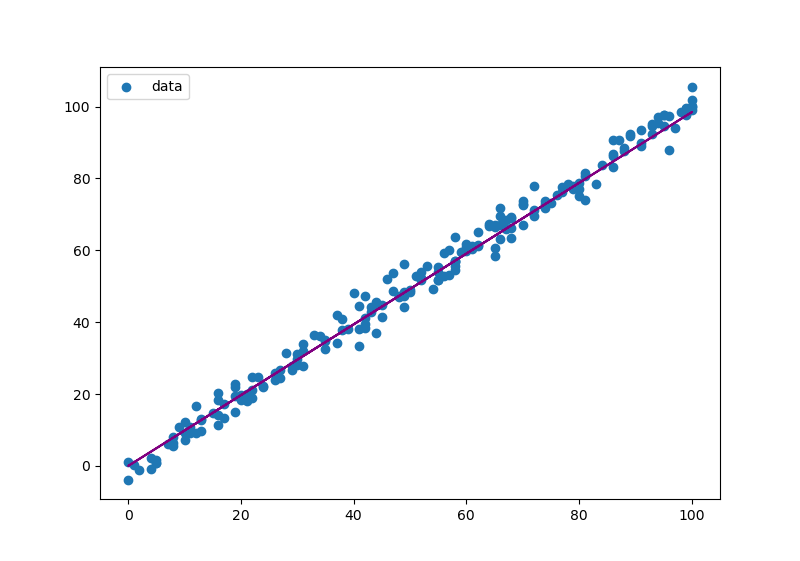
\includegraphics[width=\textwidth]{linear.png}
    \caption{Linear Regression Model}
  \end{figure}
\end{minipage}
\begin{minipage}{0.5\textwidth}
  \begin{figure}[H]
    \centering
    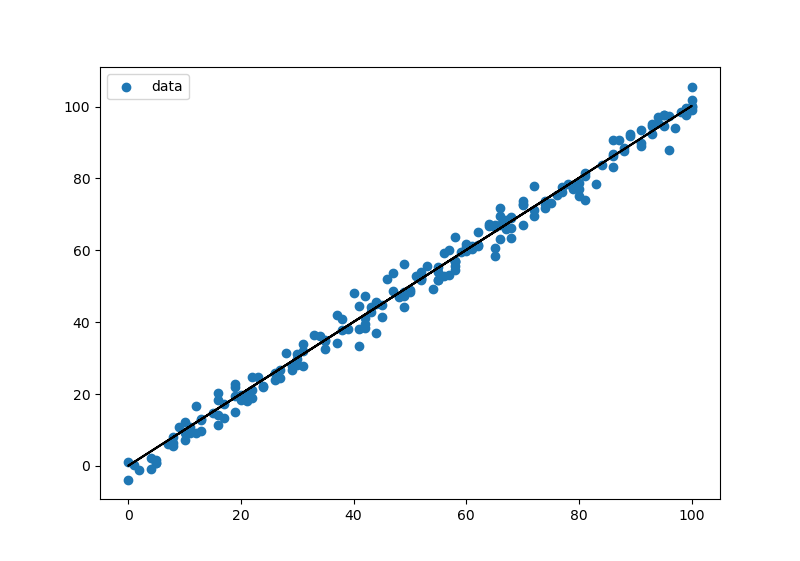
\includegraphics[width=\textwidth]{ridge.png}
    \caption{Ridge Regression Model}
  \end{figure}
\end{minipage}

\begin{figure}[H]
  \centering
  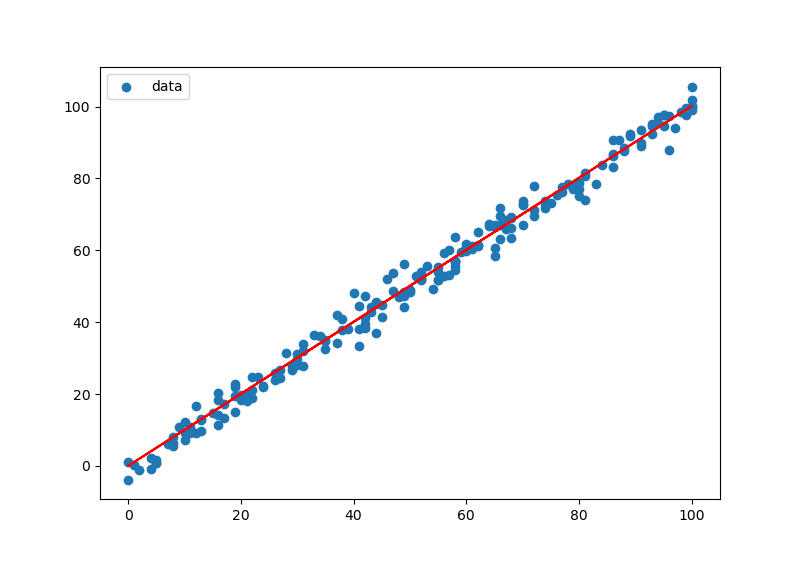
\includegraphics[width=0.5\textwidth]{best.png}
  \caption{Best performing ridge regression model with k-fold cross validation}
\end{figure}

The linear regression had a MSE of 11.74. The ridge regression had a MSE 9.60 MSE, and the best ridge regression with k-fold had a MSE of 5.98.
As we can see from the MSE values, the use of regularization in the ridge regression model improved the performance of the model.
This may be due to the original linear regression model overfitting the data, and the ridge regression model was able to perform better by penalizing complex patterns that do not generalize well.
Additionally, the use of K-fold cross validation was able significantly reduce the MSE of the ridge regression model.
This may imply that giving all of our data an equal chance to be used for training and testing has a significant impact on the performance of the model.

\end{document}